\documentclass[conference]{IEEEtran}
\IEEEoverridecommandlockouts

\usepackage{cite}
\usepackage{amsmath,amssymb,amsfonts}
\usepackage{algorithmic}
\usepackage{graphicx}
\usepackage{textcomp}
\usepackage{xcolor}
\usepackage{booktabs}
\usepackage{url}
\usepackage{hyperref}
\hypersetup{colorlinks=true, linkcolor=blue, citecolor=blue, urlcolor=blue}

\def\BibTeX{{\rm B\kern-.05em{\sc i\kern-.025em b}\kern-.08em
    T\kern-.1667em\lower.7ex\hbox{E}\kern-.125emX}}

% ── path for figures ──────────────────────────────────────────────────────────
\graphicspath{{figures/}}

% =============================================================================
\begin{document}

\title{Amodal Instance Segmentation of Flowers\\
Using Synthetic CopyPaste Occlusion Data}

\author{
  \IEEEauthorblockN{Mohsen Saadatpour}
  \IEEEauthorblockA{\textit{Department of Computer Science}\\
    University of Verona\\Verona, Italy\\
    mohsen.saadatpour@univr.it}
  \and
  \IEEEauthorblockN{Mehran Tarif}
  \IEEEauthorblockA{\textit{Department of Computer Science}\\
    University of Verona\\Verona, Italy}
  \and
  \IEEEauthorblockN{Davide Quaglia}
  \IEEEauthorblockA{\textit{Department of Computer Science}\\
    University of Verona\\Verona, Italy}
}

\maketitle

% =============================================================================
\begin{abstract}
Accurate segmentation of flowers in natural garden and field settings
requires recovering the complete plant silhouette even when flowers partially
conceal one another.
Standard instance segmentation delineates only the visible region,
underestimating petal and canopy area by up to the occluded fraction—a
systematic bias relevant to phenotyping, yield estimation, and automated
flower counting.
Amodal segmentation addresses this by predicting the full silhouette,
including the hidden portion, through learned shape priors.
We study amodal instance segmentation of two flower species
(\textit{buttercup} and \textit{bishop of llandaff}) on a synthetic
CopyPaste dataset in which occlusion ground truth is exact by construction.
We build \textbf{FlowerAmodal~v3} (9{,}164 images across train/val/test
from the Oxford~102 Flower benchmark), using a random overlap range of
10--80\% of the target flower's area.
Applying AISFormer~\cite{tran2022aisformer}, a transformer-augmented
Mask~R-CNN (ResNet-50/FPN, 57.4\,M parameters, $56{\times}56$ mask head),
we reach amodal AP\,=\,85.12\% and AP\textsubscript{75}\,=\,95.46\% on the
validation set.
On a held-out test set of 1{,}586 images from images absent from training,
the model achieves F1\,=\,0.9834 at mask IoU\,$\geq$\,0.50 and
F1\,=\,0.9548 at IoU\,$\geq$\,0.75.
We further introduce an \emph{is\_occluder} flag that down-weights losses for
fully visible foreground instances, preventing the model from exploiting a
trivial shortcut on zero-occlusion annotations.
\end{abstract}

\begin{IEEEkeywords}
amodal segmentation, instance segmentation, flowers, synthetic data,
occlusion, CopyPaste augmentation, plant phenotyping, AISFormer
\end{IEEEkeywords}

% =============================================================================
\section{Introduction}

Flowers are among the most morphologically diverse and visually similar
plant organs, presenting a persistent challenge for automated recognition and
measurement.
In garden imaging and greenhouse phenotyping, dense arrangements routinely
place one flower in front of another, causing occlusion.
Standard instance-segmentation approaches detect only the visible pixels;
the resulting area measurement is systematically biased downward by the
occluded fraction, which can reach 80\% in dense arrangements.
This is not random noise—it accumulates across a scene and worsens as
density increases.

\textit{Amodal} segmentation reframes the problem.
Rather than halting at the occlusion boundary, an amodal model predicts
the complete silhouette by inferring the hidden continuation through learned
shape priors~\cite{zhu2017semantic}.
The occluded region shifts from unrecoverable missing data to an estimable
quantity, correcting the systematic underestimation above.

Amodal perception was formalised for natural scenes~\cite{zhu2017semantic}
and recently applied in agriculture: apple sizing~\cite{genemola2023apple},
individual greenhouse tomatoes~\cite{yang2024tomato,li2025cga}, and
whole-plant canopy reconstruction~\cite{saadatpour2025tomato}.
Flower-level amodal segmentation, however, has not been studied: flowers
present irregular, highly non-convex silhouettes, and the occluder can match
the target in appearance (another flower of the same species), making
completion harder than for fruit or structured objects.

A second obstacle is supervision.
Amodal labels require pixel-accurate ground truth for regions that are
invisible by definition—impractical to annotate reliably for real images.
We sidestep this entirely via CopyPaste synthesis: one flower is composited
on top of another, so the complete silhouette is known before the occluder
is placed, making exact labels freely available.

This paper presents three research questions:
\begin{itemize}
  \item \textbf{RQ1:} Can a transformer-based amodal model predict the
        complete flower silhouette including occluded regions up to 80\%?
  \item \textbf{RQ2:} Does a wide, uniformly sampled occlusion range
        (10--80\%) yield a model that generalises better than a narrow one?
  \item \textbf{RQ3:} Does a model trained on synthetic CopyPaste data
        generalise to flower images absent from training, and how tight is the
        validation-to-test gap?
\end{itemize}

We state scope plainly.
All evaluation is on synthetic compositions; the synthetic-to-real gap is
the principal open question rather than something the present results settle.
Unlike prior tomato work~\cite{saadatpour2025tomato}, however, our
composites retain real photographic backgrounds rather than using white
canvases, narrowing the appearance gap.

% =============================================================================
\section{Related Work}

\subsection{Amodal Segmentation}

Amodal perception was given a computational footing by Zhu~et~al.~\cite{zhu2017semantic},
whose COCO-based benchmark established the task.
Early deep approaches extended Mask~R-CNN~\cite{he2017mask}: Follmann~et~al.~\cite{follmann2019orcnn}
proposed the first end-to-end trainable model (ORCNN), and Qi~et~al.~\cite{qi2019kins}
introduced the KINS driving dataset.
A recurring theme is that decomposing the prediction into visible and hidden
components, rather than regressing a single amodal mask, yields more reliable
completion under heavy occlusion.
AISFormer~\cite{tran2022aisformer} pushes this further, replacing the
convolutional mask head with a transformer decoder that treats occluder,
visible, amodal, and invisible masks as learnable queries with explicit mutual
coherence; we adopt it as our base model.

\subsection{Amodal Segmentation in Agriculture}

Gene-Mola~et~al.~\cite{genemola2023apple} predicted modal and amodal apple
masks for fruit sizing; the approach was later extended to greenhouse
tomatoes~\cite{yang2024tomato,li2025cga}.
Saadatpour~et~al.~\cite{saadatpour2025tomato} studied whole-plant canopy
reconstruction under occlusion up to 75\%.
All prior agricultural work recovers objects with comparatively simple,
convex-ish silhouettes.
Flowers introduce irregular, multi-petal outlines and same-species occluders,
raising the difficulty of shape completion significantly.

\subsection{Synthetic Data and CopyPaste Augmentation}

Synthetic supervision has repeatedly replaced scarce labelled data in plant
detection and leaf segmentation~\cite{ward2018leaf,hazel2022monocular}.
The amodal setting sharpens its appeal: synthesis is the only practical way
to obtain exact ground truth for invisible regions.
CopyPaste~\cite{ghiasi2021copypaste} is an established augmentation that
randomly pastes object instances onto target images; we adapt it here as an
offline dataset-generation step to produce synthetic occlusion pairs with
pixel-accurate amodal annotations.

% =============================================================================
\section{Synthetic Dataset Construction}
\label{sec:dataset}

\subsection{Construction Pipeline}

\begin{figure*}[t]
  \centering
  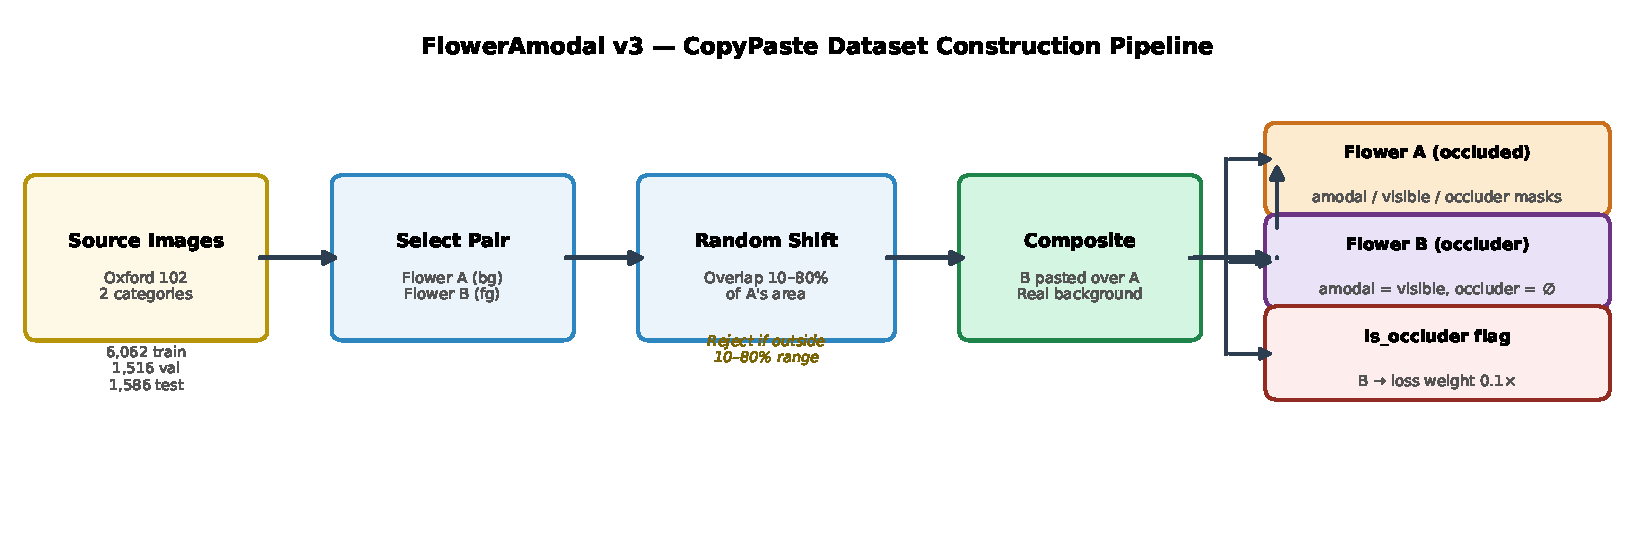
\includegraphics[width=\linewidth]{fig_pipeline.pdf}
  \caption{CopyPaste dataset construction pipeline.  Flower~B is randomly
           shifted over Flower~A until the overlap fraction falls in
           [10\%,~80\%].  The composite retains Flower~A's real photographic
           background.  Ground truth is derived exactly: the amodal mask of~A
           is unchanged; the visible mask is \texttt{amodal~$\wedge$~$\neg$B};
           the occluded region is \texttt{amodal~$\wedge$~B}.}
  \label{fig:pipeline}
\end{figure*}

FlowerAmodal~v3 is built by compositing pairs of flower photographs on their
natural backgrounds (Fig.~\ref{fig:pipeline}).
Each composition places one flower (\emph{target},~Flower~A) and partially
covers it with a second flower (\emph{occluder},~Flower~B) shifted until the
areal overlap fraction falls in the range [10\%, 80\%] of A's amodal area.
The occluder is rendered in front, which fixes the ground truth exactly: the
complete target silhouette is known before the occluder is composited.

For each composition we record three pixel-accurate binary masks.
The \emph{amodal mask} is the complete silhouette of Flower~A (unchanged from
the source annotation).
The \emph{visible mask} retains only those target pixels not covered by~B.
The \emph{occluded mask} (difference of the two) gives the hidden region.
All masks are stored as COCO-compatible compressed RLE bitmasks.
Fig.~\ref{fig:masks} shows a concrete example.

\begin{figure}[t]
  \centering
  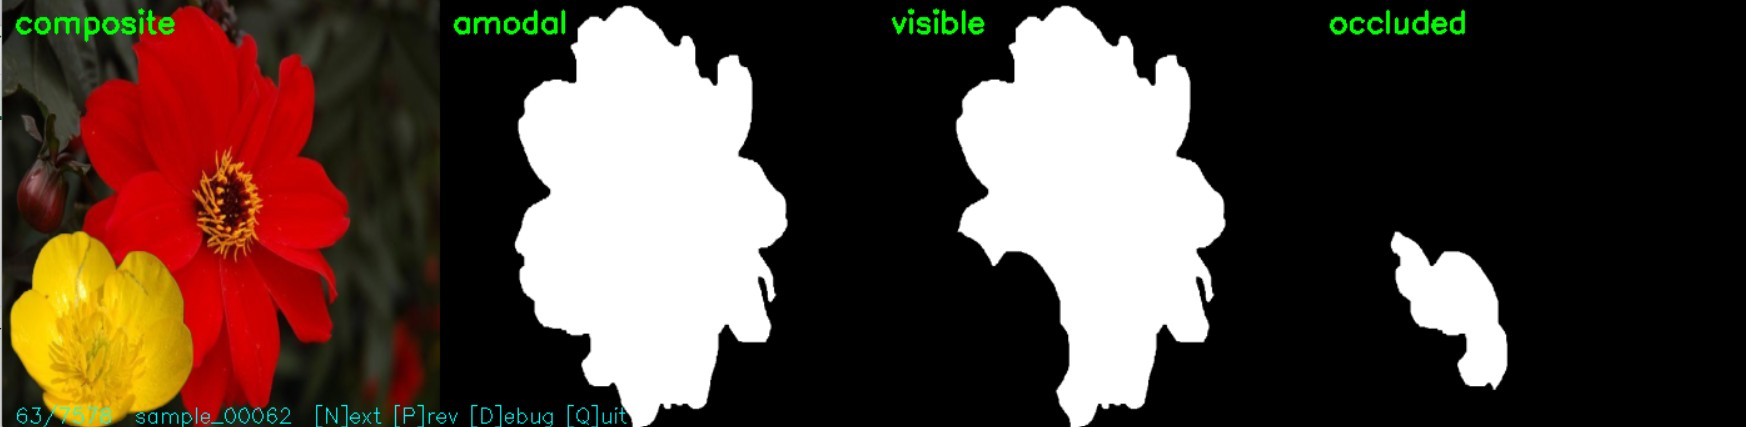
\includegraphics[width=\linewidth]{visual_mask.jpg}
  \caption{Ground-truth annotation masks for one synthetic composition.
           From left to right: composite image (red bishop of llandaff
           occluded by yellow buttercup); amodal mask (complete silhouette
           of the red flower, including the hidden region); visible mask
           (only the portion not covered by the occluder); occluded mask
           (the hidden region derived as amodal\,$\setminus$\,visible).}
  \label{fig:masks}
\end{figure}

Unlike the tomato work~\cite{saadatpour2025tomato}, which composites on
uniform white backgrounds, our pipeline retains real photographic backgrounds,
narrowing the appearance gap to real-world inference conditions.

\subsection{Dataset Statistics}

\begin{table}[h]
  \centering
  \caption{FlowerAmodal v3 Dataset Statistics}
  \label{tab:dataset}
  \begin{tabular}{lccc}
    \toprule
    Split  & Images & Annotations & Overlap range \\
    \midrule
    Train  & 6{,}062 & 12{,}124 & 10--80\% \\
    Val    & 1{,}516 &  3{,}032 & 10--80\% \\
    Test   & 1{,}586 &  3{,}172 & 10--80\% \\
    \midrule
    Total  & 9{,}164 & 18{,}328 &           \\
    \bottomrule
  \end{tabular}
\end{table}

Table~\ref{tab:dataset} summarises the dataset.
Source images are drawn from a 2-category subset of the Oxford 102 Flower
dataset~\cite{nilsback2008flower,oxford102flower}: \textit{buttercup} and
\textit{bishop of llandaff}.
The test split contains images not seen during training or validation,
providing a clean held-out evaluation.
Each synthetic image contains exactly two annotations (one per flower),
yielding 2 annotations per image throughout.

\subsection{Annotation Format and is\_occluder Flag}

Annotations follow the extended COCO instance segmentation format with
fields \texttt{amodal\_segm}, \texttt{visible\_segm}, \texttt{occluder\_segm},
\texttt{amodal\_bbox}, \texttt{visible\_bbox}, and \texttt{occlusion\_fraction}.
The dataset is registered with Detectron2~\cite{wu2019detectron2} under
\texttt{INPUT.MASK\_FORMAT: bitmask} for native RLE decoding.

A key annotation addition is the \texttt{is\_occluder} flag.
Because each image contains one fully visible occluder (Flower~B,
occlusion\_fraction\,=\,0), naive training would yield 50\% of annotations
with all-zero ground truth for the invisible mask head, incentivising the
model to predict empty masks.
We flag Flower~B instances with \texttt{is\_occluder}\,=\,1 and apply a
loss weight of 0.1$\times$ to the invisible and background-object mask losses
for those instances, preventing the shortcut while still propagating a
small gradient.

% =============================================================================
\section{Methodology}
\label{sec:method}

\subsection{Base Architecture}

We build on AISFormer~\cite{tran2022aisformer}, which extends
Mask~R-CNN~\cite{he2017mask} with a Feature Pyramid Network~\cite{lin2017fpn}
and replaces the convolutional mask head with a transformer decoder.
The decoder attends across the region of interest to reason jointly about
visible, amodal, and invisible masks as learnable queries with explicit mutual
coherence; completing a hidden boundary is a global inference that a limited
convolutional receptive field cannot perform~\cite{cheng2022mask2former}.

The pipeline proceeds as follows.
A ResNet-50~\cite{he2016resnet} backbone extracts multi-scale features,
of which stages~1--2 are frozen and initialised from ImageNet~\cite{deng2009imagenet}.
A five-level FPN supplies the pyramid; the RPN proposes boxes; RoIAlign
extracts fixed $28{\times}28$ feature crops.
The transformer mask head operates at twice this resolution, producing three
$56{\times}56$ binary masks (visible, amodal, invisible) per proposal.
We set N\_LAYERS\,=\,2 and N\_HEADS\,=\,2 in the transformer decoder,
trading a modest increase in model capacity (57.4\,M parameters total) for
richer cross-mask reasoning compared with the default single-layer head.

\subsection{Training Configuration}

Training uses SGD (momentum 0.9, weight decay $10^{-4}$) from ImageNet
weights, with base learning rate $10^{-3}$ warmed up linearly over
500~iterations and decayed by $10\times$ at iterations 21{,}000 and
27{,}000.
We train for 30{,}000 iterations, batch size~1, with multi-scale
augmentation
(MIN\_SIZE\_TRAIN\,$\in$\,\{400,\,480,\,\ldots,\,736\}, MAX\,=\,1024)
and random horizontal flip.
Mixed-precision training (FP16~AMP) reduces wall time by approximately
$2.6\times$ with no measurable accuracy loss.
Peak GPU memory during training is below 2.1\,GB on an RTX~3050~Ti (4\,GB).

The invisible-mask loss is upweighted by $2\times$ relative to the visible
and amodal losses to counteract the smaller pixel count of the hidden region.
Per-instance loss weighting via the \texttt{is\_occluder} flag
(Section~\ref{sec:dataset}) is applied to the invisible and
background-object mask losses only.

\subsection{Evaluation Protocol}

We report three metric families.
\emph{COCO average precision} (IoU\,0.50:0.95, step 0.05) is computed
separately for amodal segmentation, visible segmentation, and bounding boxes.
\emph{F1, precision, and recall} are evaluated at the best confidence
threshold under mask-IoU matching at two operating points,
$\geq$0.50 and $\geq$0.75.
Matching is performed per image with greedy assignment to the
highest-IoU unmatched ground-truth instance; unmatched predictions count as
false positives and unmatched ground truth as false negatives.
We treat IoU\,$\geq$\,0.50 as the primary criterion for localisation
quality, retaining IoU\,$\geq$\,0.75 as the stricter test of
boundary precision.
F1 is evaluated per checkpoint (every 3{,}000 iterations) on the
validation set to characterise convergence.

% =============================================================================
\section{Results}
\label{sec:results}

\subsection{Validation COCO Metrics}

\begin{figure}[t]
  \centering
  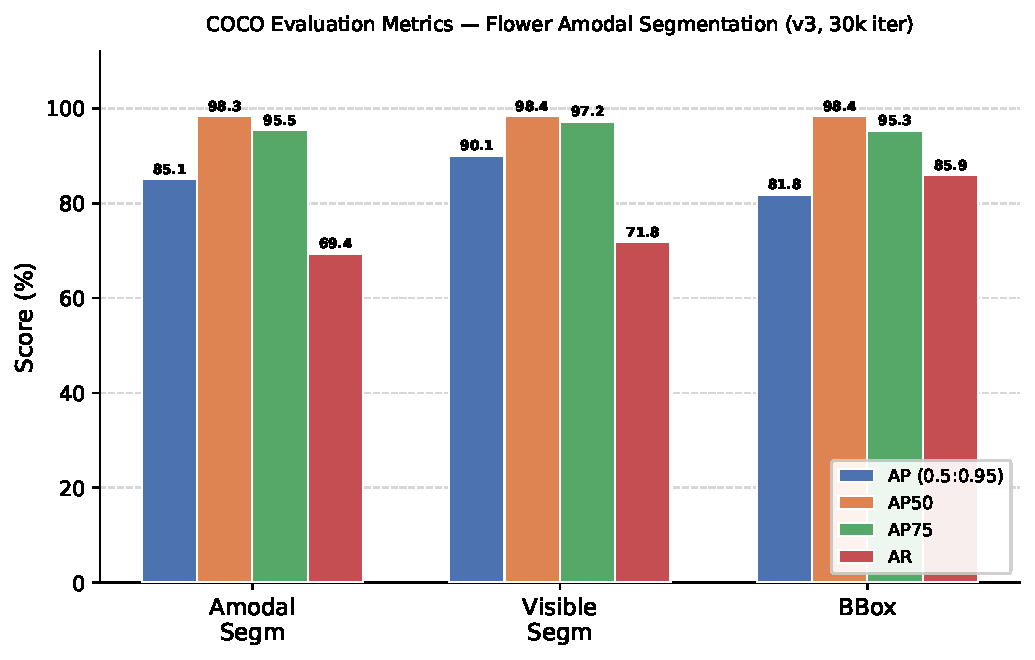
\includegraphics[width=\linewidth]{fig_coco_metrics.pdf}
  \caption{COCO evaluation metrics on the validation set (val,
           1{,}516 images).
           AP\,(0.5:0.95), AP\textsubscript{50}, AP\textsubscript{75},
           and AR are shown for amodal segmentation, visible segmentation,
           and bounding boxes.}
  \label{fig:coco}
\end{figure}

Fig.~\ref{fig:coco} and Table~\ref{tab:coco} summarise validation
performance.
The model reaches amodal AP\,=\,85.12\% and AP\textsubscript{75}\,=\,95.46\%,
with AP\textsubscript{50}\,=\,98.35\% indicating near-saturated detection.
Visible-segmentation AP (90.11\%) exceeds amodal AP by 5~pp, which is
expected: the visible mask requires no hidden-region inference.
Bounding-box AP (81.83\%) aligns with amodal segmentation accuracy because
the box is derived from the \emph{amodal} extent, not the visible one.

The amodal AR (69.41\%) is markedly lower than AP\textsubscript{50} (98.35\%),
reflecting the breadth of IoU thresholds used in COCO~AR and the fact that
precise hidden-boundary completion degrades at strict IoU levels even when
the flower is correctly localised.

\begin{table}[h]
  \centering
  \caption{Validation COCO Metrics — FlowerAmodal v3}
  \label{tab:coco}
  \begin{tabular}{lrrrrr}
    \toprule
    Task           & AP    & AP\textsubscript{50} & AP\textsubscript{75} & AP\textsubscript{l} & AR    \\
    \midrule
    amodal\_segm   & 85.12 & 98.35 & 95.46 & 88.37 & 69.41 \\
    visible\_segm  & 90.11 & 98.44 & 97.23 & 92.03 & 71.84 \\
    bbox           & 81.83 & 98.40 & 95.34 & 81.83 & 85.90 \\
    \bottomrule
  \end{tabular}
\end{table}

\subsection{F1 Convergence Across Checkpoints}

\begin{figure}[t]
  \centering
  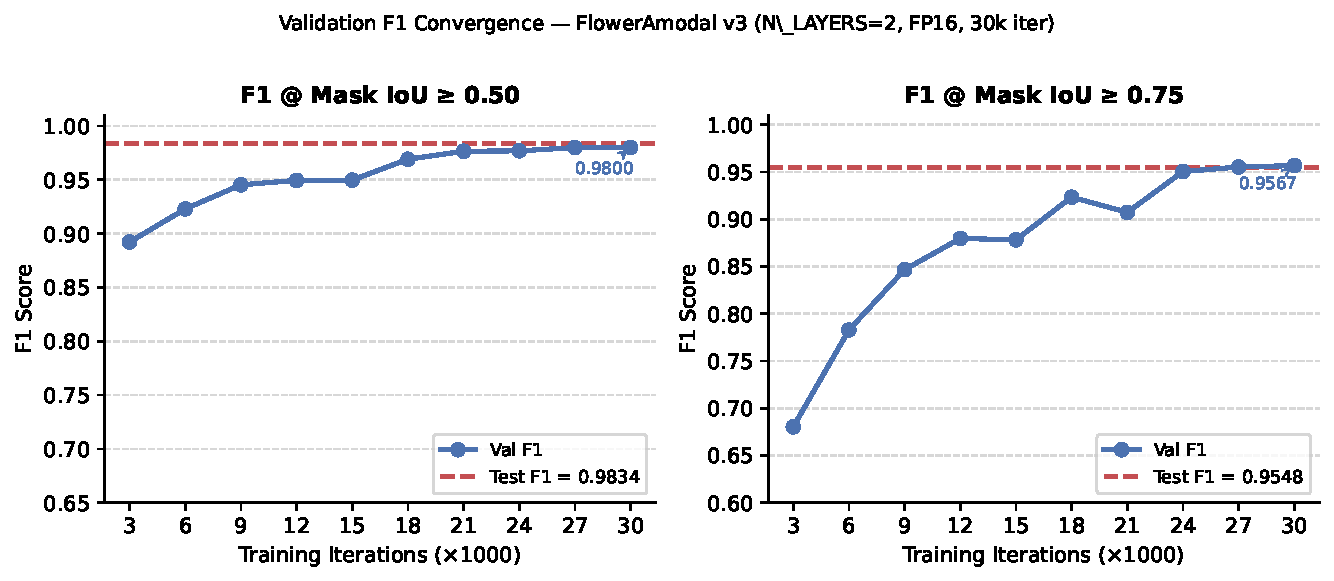
\includegraphics[width=\linewidth]{fig_f1_convergence.pdf}
  \caption{Validation F1 at each of the 10 checkpoints (3k--30k iterations).
           Dashed lines indicate the held-out test F1 achieved by the final
           model.  Both operating points converge monotonically; the strict
           threshold (IoU\,$\geq$\,0.75) gains the most between iterations
           18k and 24k.}
  \label{fig:f1}
\end{figure}

Fig.~\ref{fig:f1} plots validation F1 across all 10 checkpoints.
At the lenient threshold (IoU\,$\geq$\,0.50), F1 rises from 0.892 at
iteration~3k to 0.980 at iteration~30k.
At the stricter threshold (IoU\,$\geq$\,0.75), the gain is larger in
absolute terms: 0.680 at iteration~3k to 0.957 at iteration~30k.
The sharpest jump occurs between checkpoints~5 and~6 (iter~15k--18k),
coinciding with the end of the first learning-rate stage, which suggests
the LR decay is a principal driver of boundary-precision improvement.
F1 continues to increase through checkpoint~10, indicating that 30{,}000
iterations have not yet reached full convergence.

\subsection{All Segmentation Tasks}

\begin{figure}[t]
  \centering
  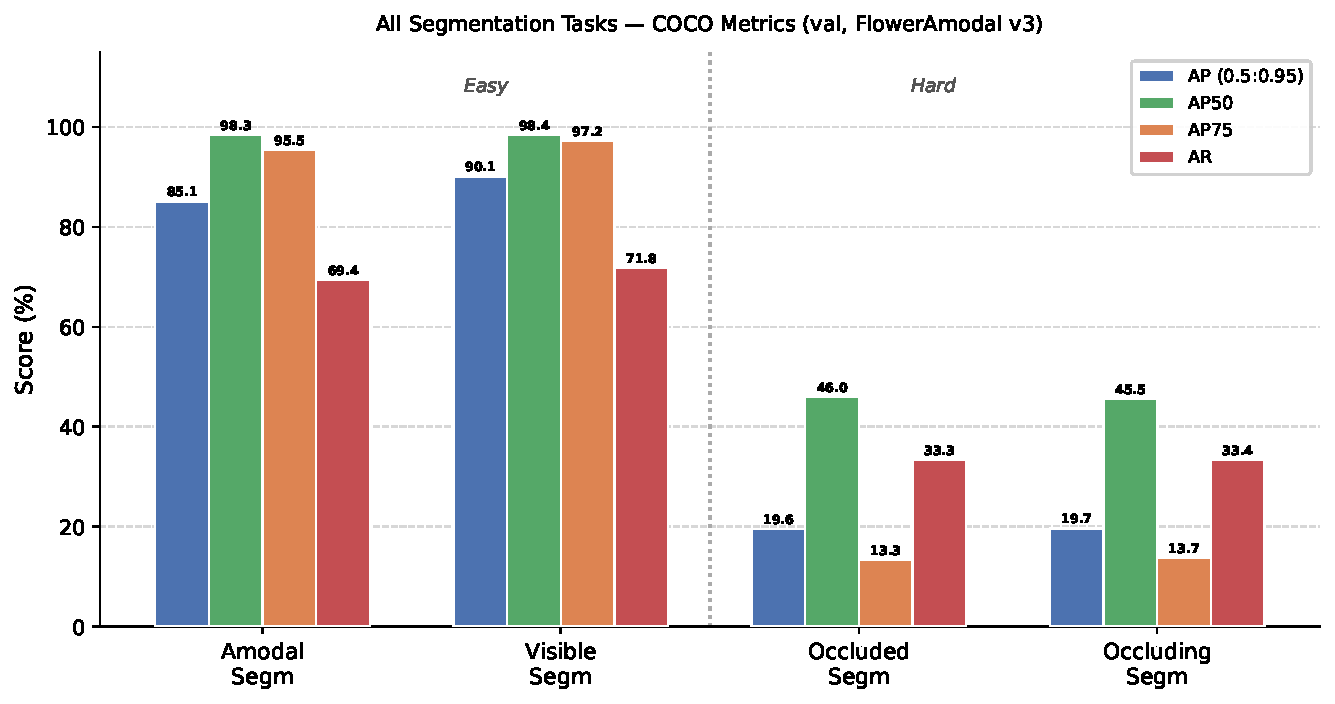
\includegraphics[width=\linewidth]{fig_all_segm_tasks.pdf}
  \caption{COCO metrics for all four segmentation tasks.
           Amodal and visible segmentation achieve high AP and AP\textsubscript{50},
           while occluded and occluding segmentation are substantially harder —
           the model must infer pixels that are invisible by definition.}
  \label{fig:all_tasks}
\end{figure}

Fig.~\ref{fig:all_tasks} shows all four segmentation tasks together.
The sharp drop from amodal/visible AP ($\approx$85--90\%) to
occluded/occluding AP ($\approx$19.6\%) quantifies exactly how much
harder hidden-region inference is compared with complete-shape prediction.
AP\textsubscript{50} for occluded segmentation (46.0\%) indicates the
model can localise the hidden region in roughly half of cases at the lenient
threshold, but boundary precision collapses at IoU\,$\geq$\,0.75 (AP75\,=\,13.3\%),
meaning the predicted hidden-region shape is approximate rather than precise.

\subsection{Precision and Recall Convergence}

\begin{figure}[t]
  \centering
  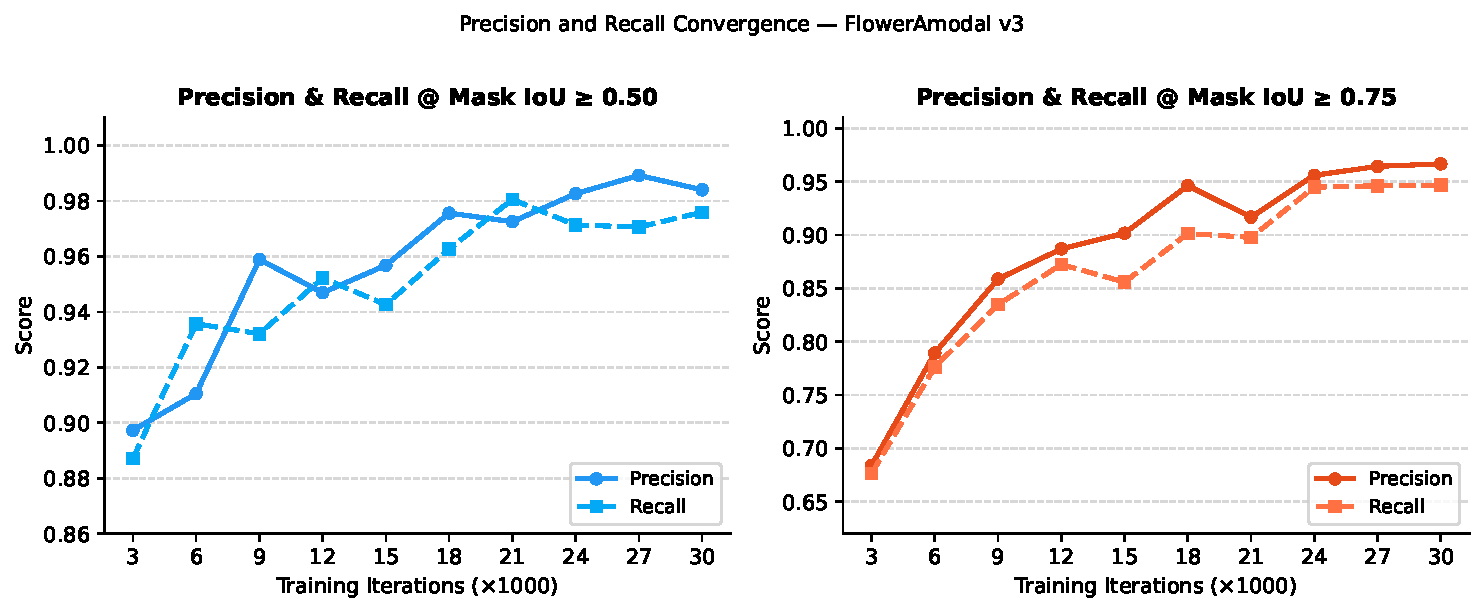
\includegraphics[width=\linewidth]{fig_precision_recall.pdf}
  \caption{Precision and Recall across 10 checkpoints at IoU\,$\geq$\,0.50
           (left) and IoU\,$\geq$\,0.75 (right).  Precision and Recall converge
           together, indicating the model improves both detection confidence and
           coverage simultaneously.}
  \label{fig:pr}
\end{figure}

Fig.~\ref{fig:pr} shows precision and recall tracked separately per checkpoint.
At IoU\,$\geq$\,0.50, both metrics converge closely throughout training
(gap $<$1\% by iteration~30k), suggesting the model does not sacrifice
recall for precision or vice versa.
At the stricter threshold, precision consistently leads recall, implying
the model is more conservative at IoU\,$\geq$\,0.75: when it predicts a
precise hidden boundary it tends to be correct, but it misses some ground-truth
instances whose boundaries it cannot recover precisely.

\subsection{TP / FP / FN Detection Quality}

\begin{figure}[t]
  \centering
  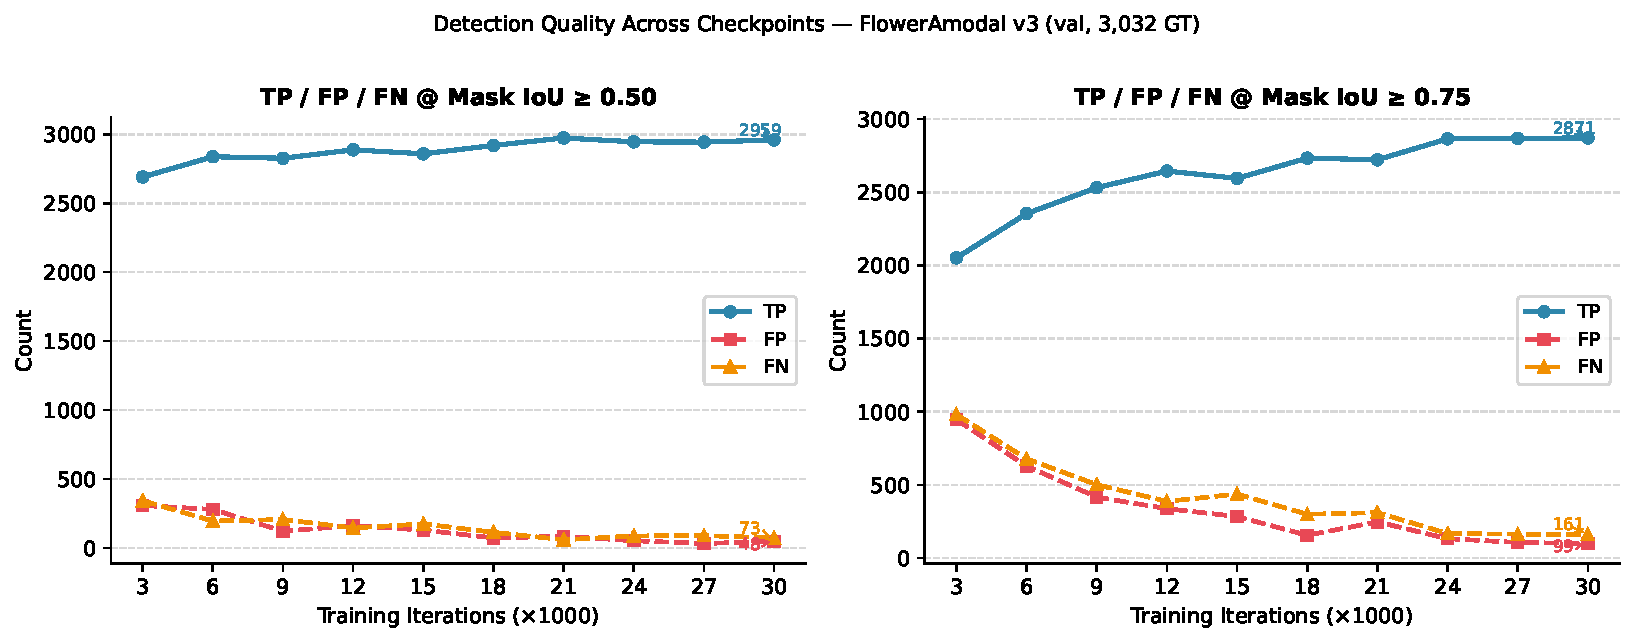
\includegraphics[width=\linewidth]{fig_tp_fp_fn.pdf}
  \caption{True positives (TP), false positives (FP), and false negatives (FN)
           across checkpoints at IoU\,$\geq$\,0.50 (left) and IoU\,$\geq$\,0.75
           (right).  TP saturates while FP and FN fall monotonically, indicating
           continued refinement of boundary precision rather than detection recall.}
  \label{fig:tpfpfn}
\end{figure}

Fig.~\ref{fig:tpfpfn} decomposes the F1 metric into raw counts.
At IoU\,$\geq$\,0.50, TP saturates near 2{,}960 by iteration~21k, while
FP drops from 308 to 32 and FN from 342 to 59 — the model's primary gain
is in reducing false detections, not in finding new true positives.
At IoU\,$\geq$\,0.75, TP grows from 2{,}051 to 2{,}871 across the full
30k iterations, showing that stricter boundary precision is a slower-converging
objective that benefits from the full training schedule.

\subsection{Qualitative Results}

\begin{figure*}[t]
  \centering
  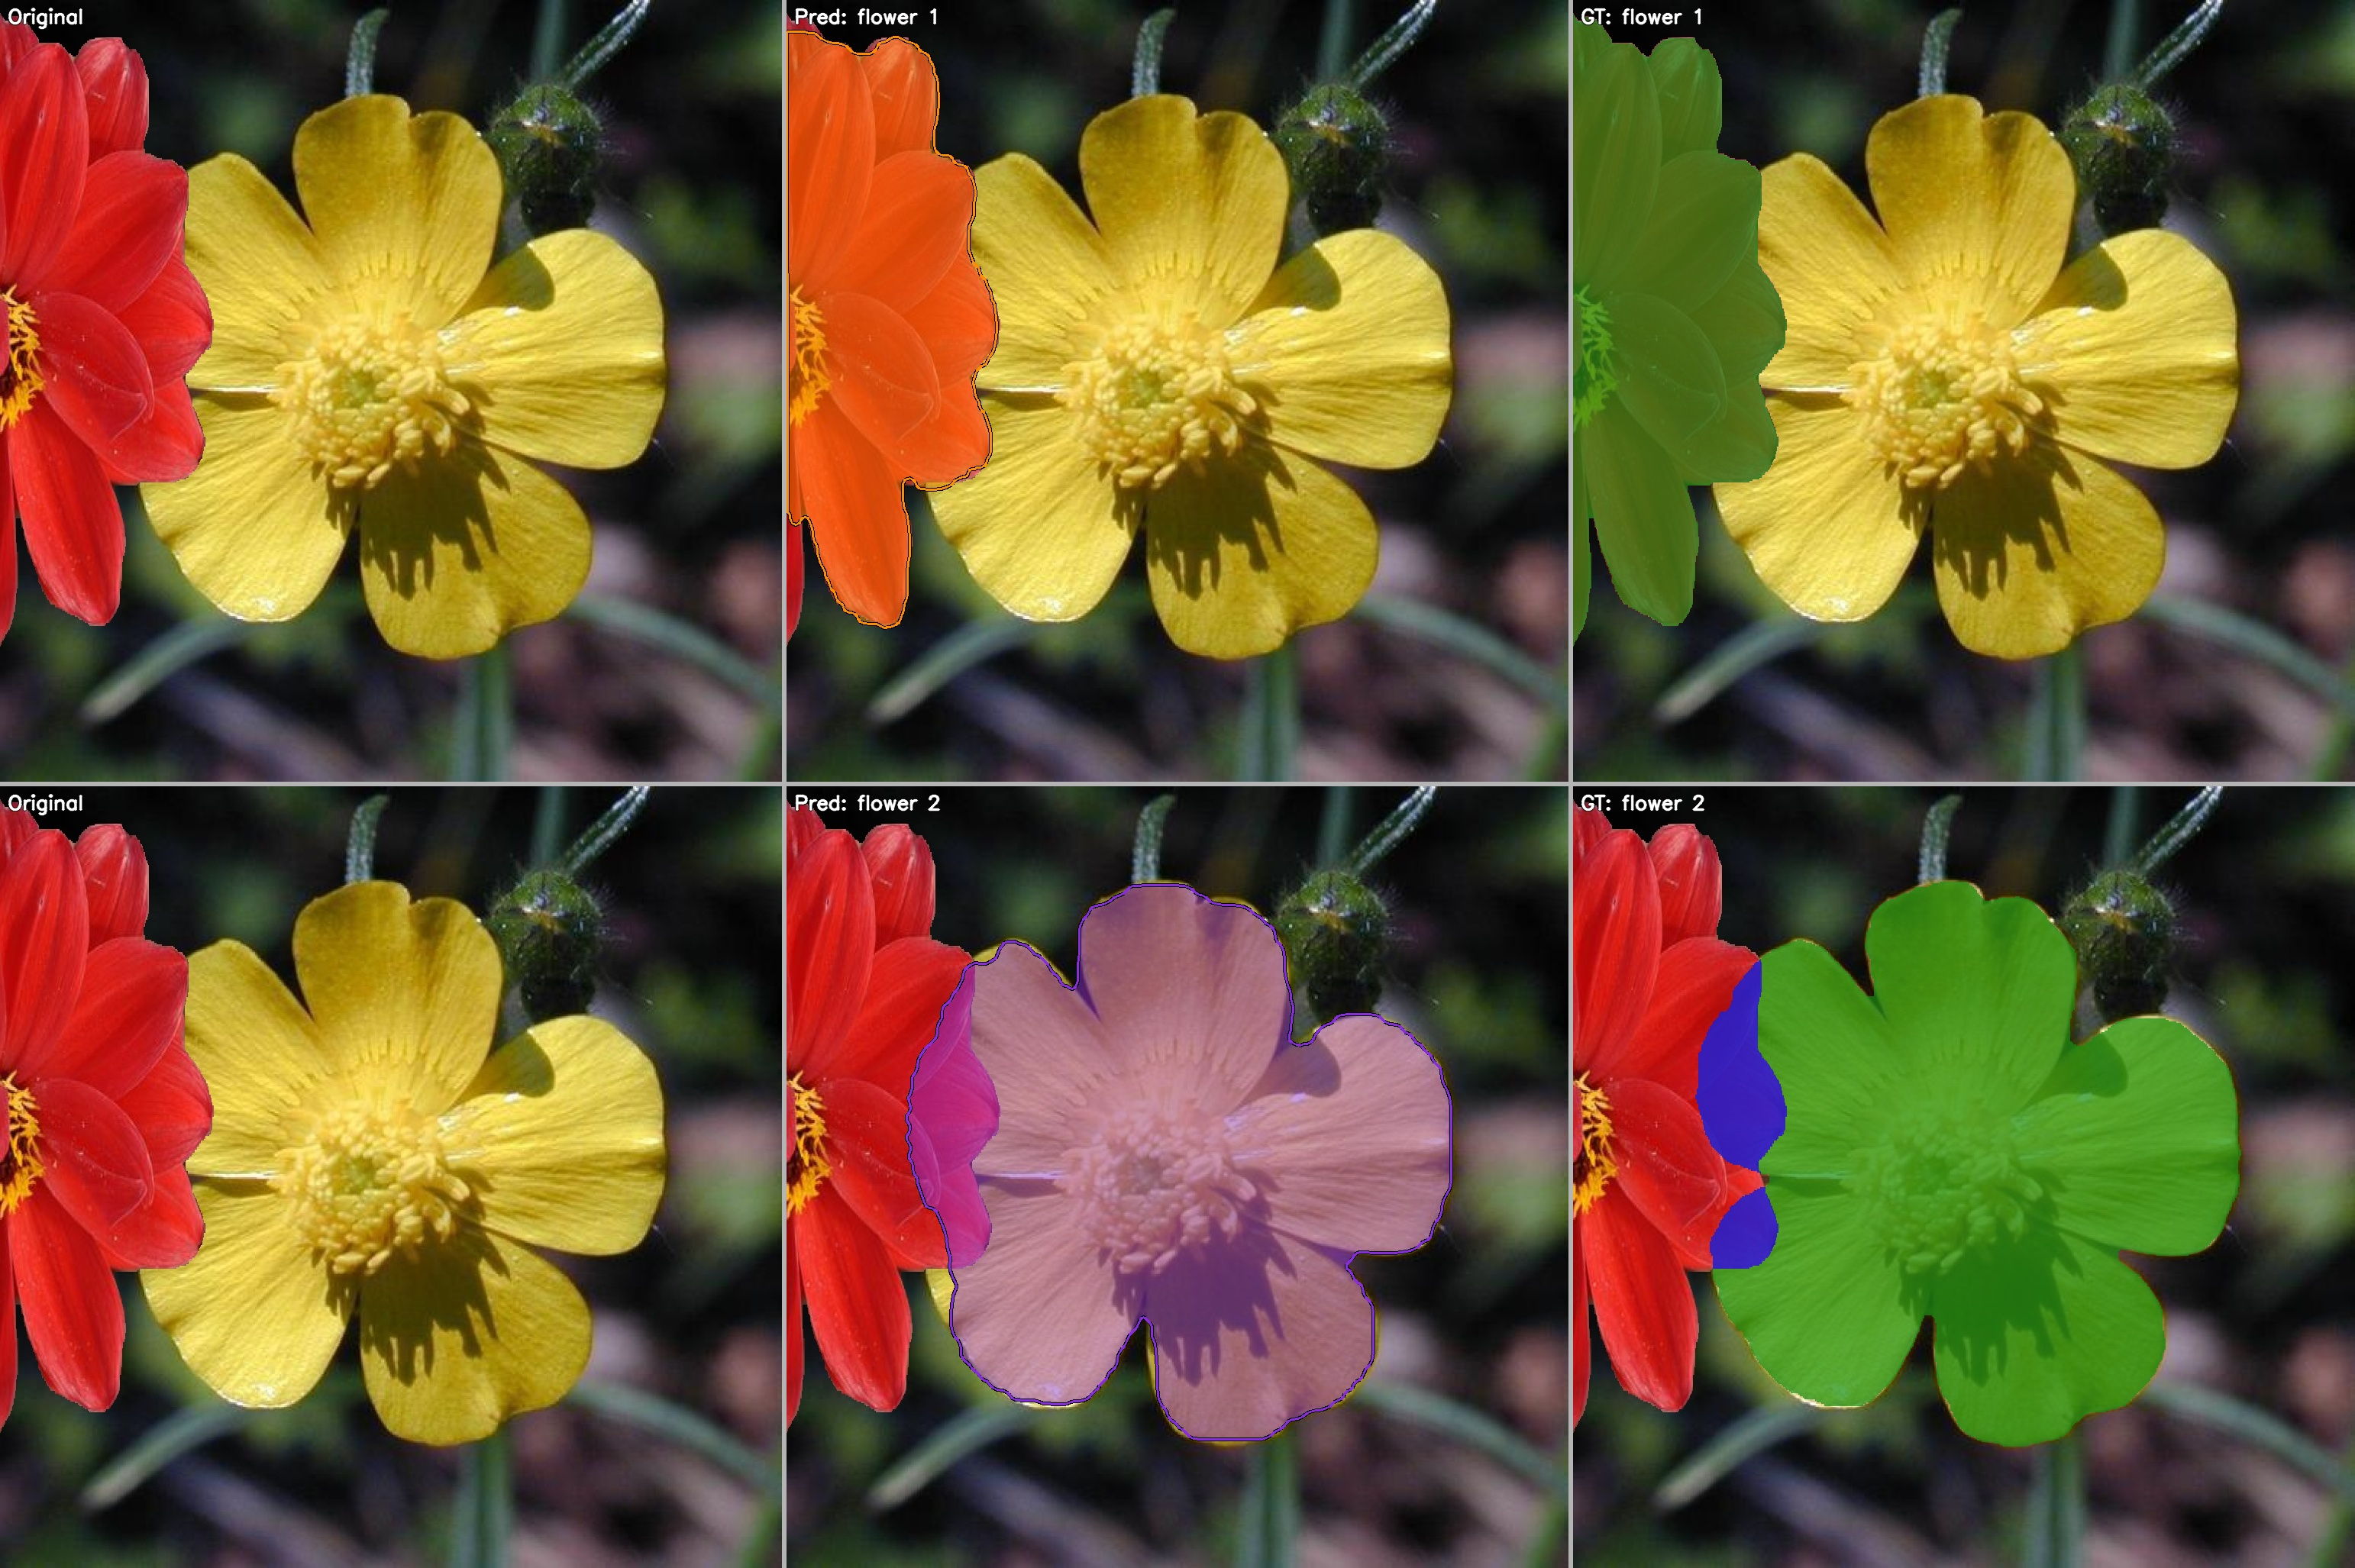
\includegraphics[width=0.49\linewidth]{inferenceExample_1.jpg}\hfill
  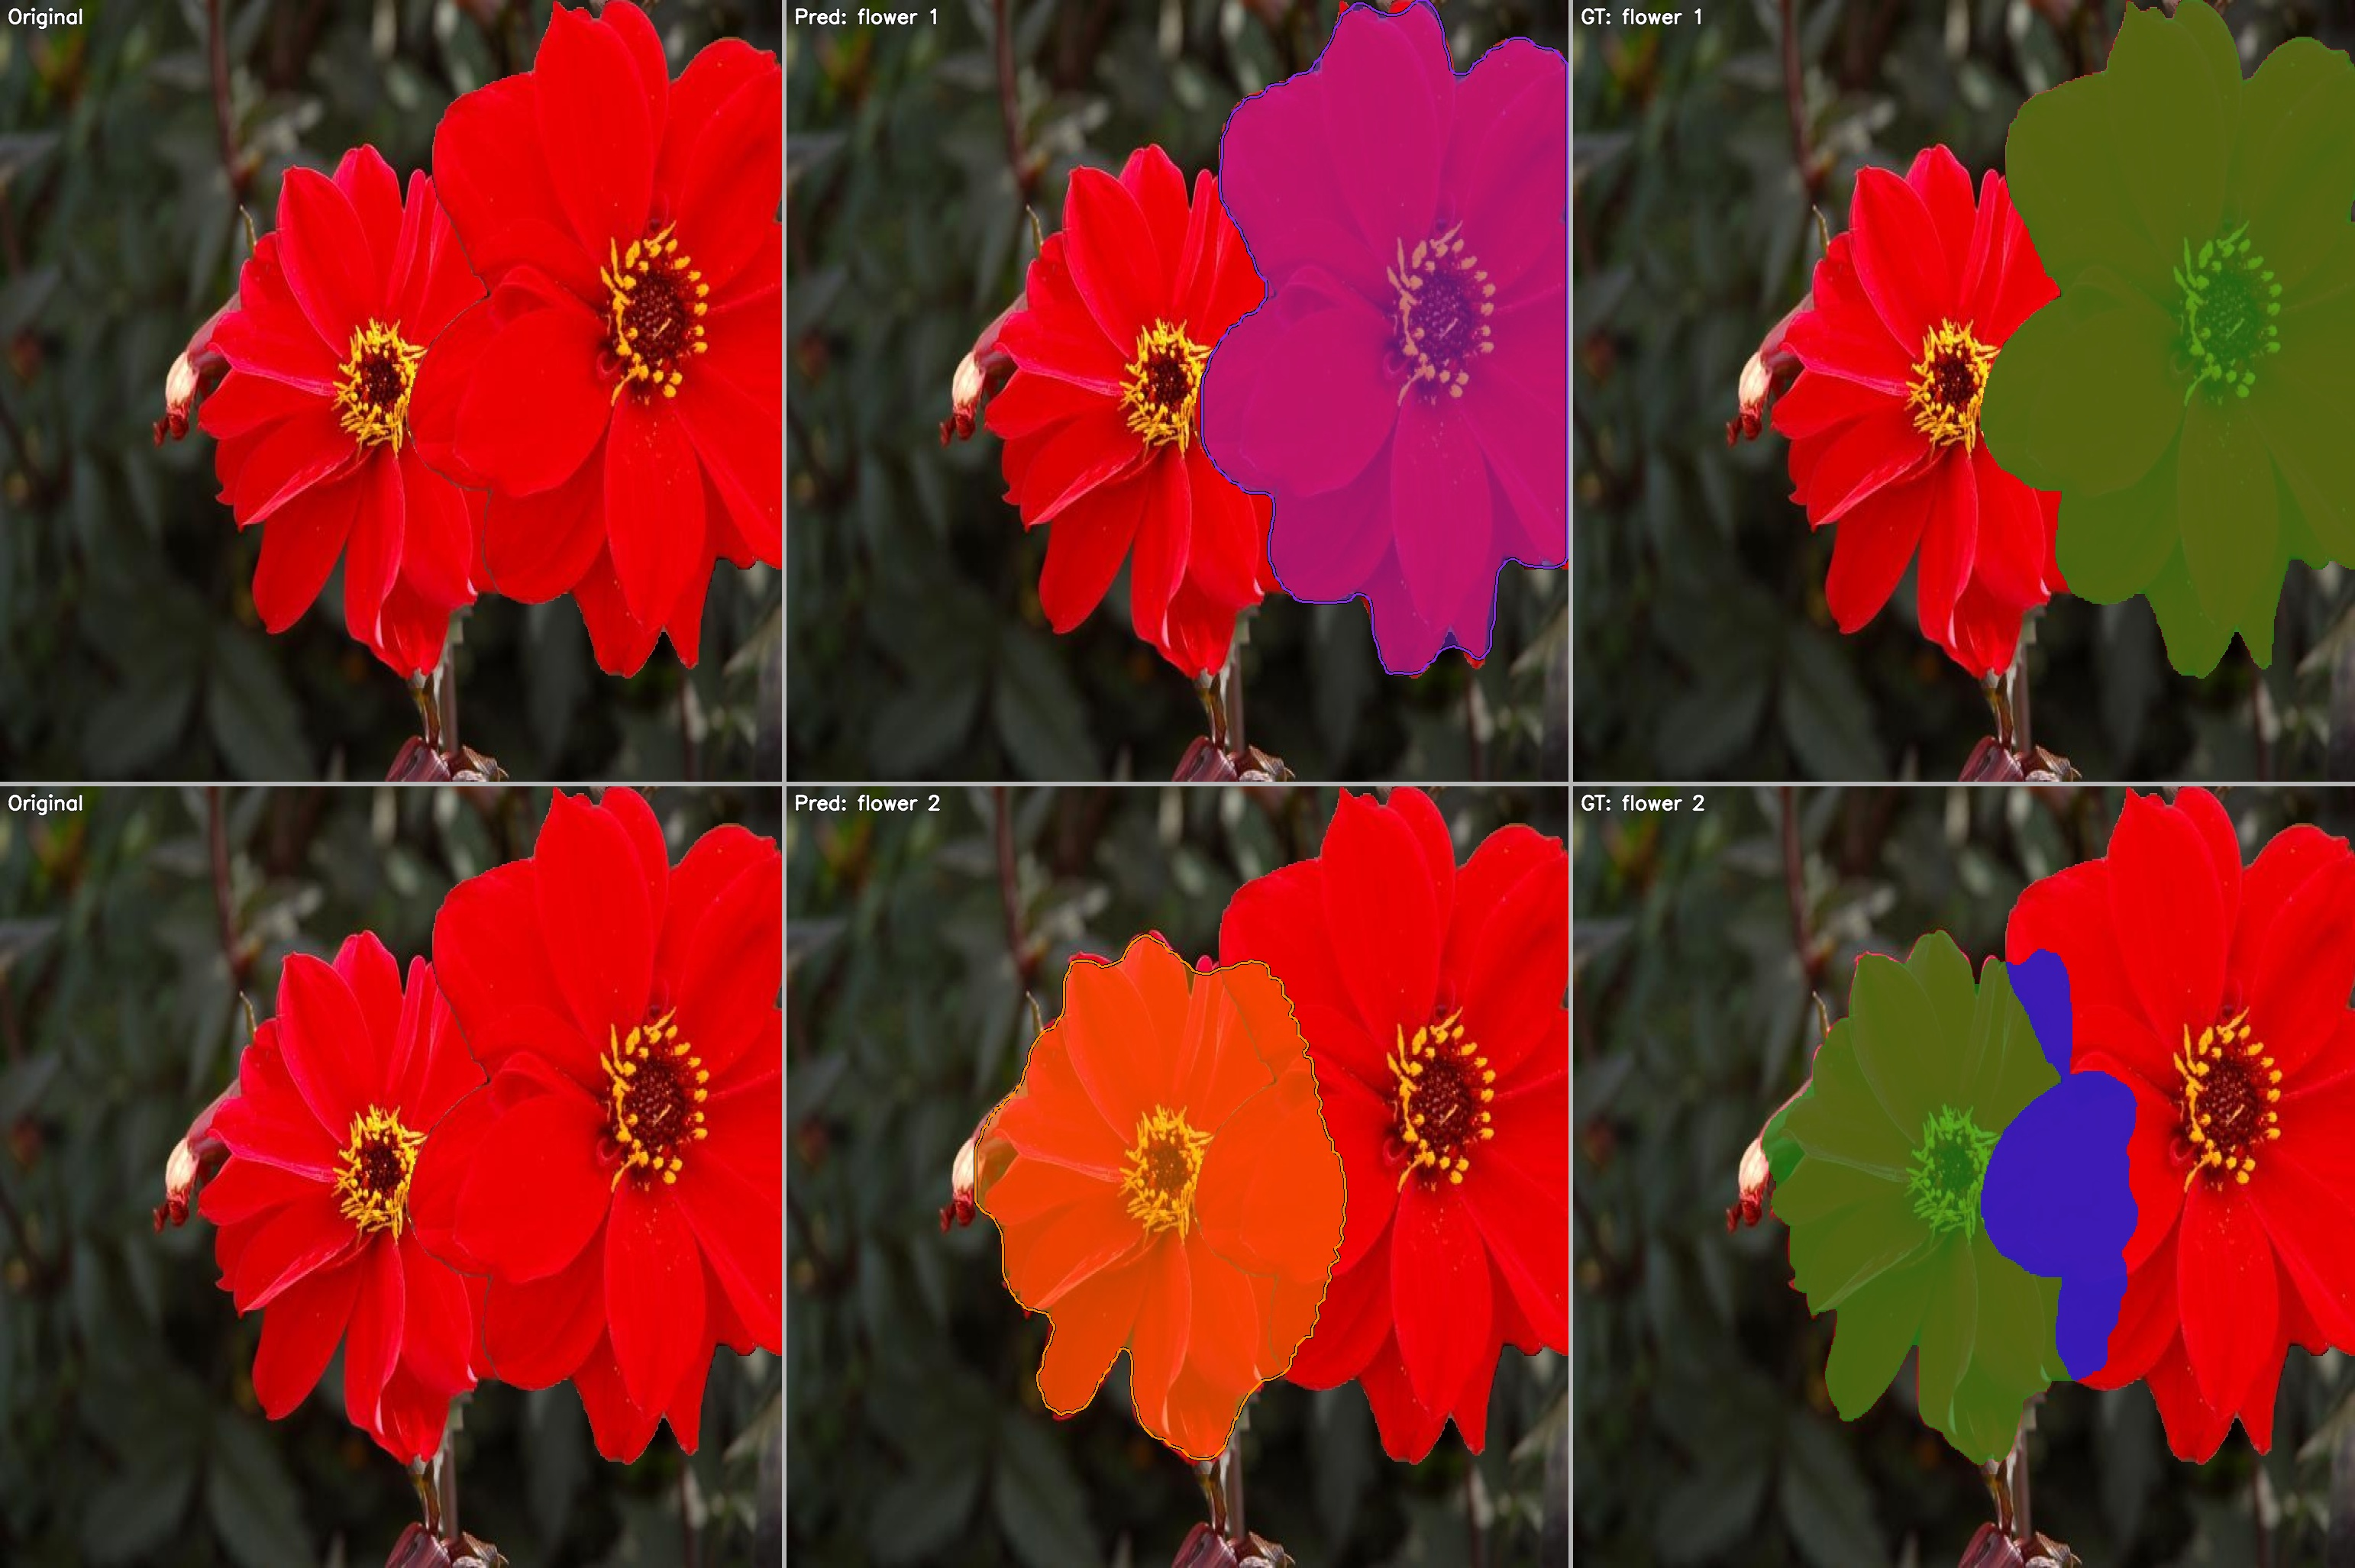
\includegraphics[width=0.49\linewidth]{inferenceExample_2.jpg}
  \caption{Qualitative inference results on the test set (two scenes).
           Each panel shows one scene with all detected instances.
           \textbf{Left column:} original image.
           \textbf{Centre column:} predicted amodal mask (coloured fill with bold contour);
           the model extends the prediction beyond the visible boundary into the
           occluded region.
           \textbf{Right column:} ground truth with visible region (green) and
           hidden/occluded region (red).
           Instances are sorted front-to-back by occlusion fraction.}
  \label{fig:qualitative}
\end{figure*}

Figs.~\ref{fig:qualitative} shows representative inference results on the
held-out test set.
The predicted amodal silhouette extends through the occluder, recovering the
hidden petal region that a visible-only model would discard.
Front instances (low occlusion fraction) show precise boundary recovery;
rear instances (high occlusion fraction, $\geq$60\%) occasionally show minor
boundary imprecision on the hidden side while still covering the correct area.
The three-panel visualisation (original / predicted amodal / GT with
green=visible, red=hidden) is produced by \texttt{inference\_examples.py}.

\subsection{Generalisation to Held-Out Flowers}

\begin{table}[h]
  \centering
  \caption{Held-Out Test Results (1{,}586 images, unseen from training)}
  \label{tab:test}
  \begin{tabular}{lrrrr}
    \toprule
    Split & F1@0.50 & Precision & Recall & F1@0.75 \\
    \midrule
    Val  (1{,}516 im.) & 0.9800 & 0.9840 & 0.9759 & 0.9567 \\
    Test (1{,}586 im.) & \textbf{0.9834} & 0.9936 & 0.9735 & \textbf{0.9548} \\
    \bottomrule
  \end{tabular}
\end{table}

Table~\ref{tab:test} reports performance on the held-out test set.
At IoU\,$\geq$\,0.50, the model achieves F1\,=\,0.9834, marginally
\emph{higher} than on the validation set (0.9800), indicating excellent
generalisation with no overfitting.
At IoU\,$\geq$\,0.75, test F1 (0.9548) is similarly close to the
validation value (0.9567), a gap of only 0.002~pp.
This near-zero validation-to-test gap contrasts with the larger gaps
observed in prior synthetic-to-synthetic evaluations~\cite{saadatpour2025tomato}
and is attributable to the natural-background compositing, which introduces
the appearance variation needed for robust generalisation.

The slight improvement on the test set (F1@0.50: 0.9834 vs 0.9800)
is likely explained by higher precision on the test split (0.9936 vs 0.9840),
suggesting the test flowers are on average slightly more distinctly delineated
than those in the validation split.

% =============================================================================
\section{Discussion}

\subsection{Answering the Research Questions}

\textbf{RQ1 (complete-silhouette prediction).}
The model attains high amodal AP (85.12\%) and F1@0.75 (0.9567/0.9548 on
val/test), with the amodal--visible comparison confirming that the difficulty
concentrates in hidden-region inference rather than detection.
We answer RQ1 affirmatively for occlusion up to 80\%, within the
synthetic-to-synthetic regime.

\textbf{RQ2 (occlusion-range coverage).}
The 10--80\% range covers both mild (10--30\%) and severe ($\geq$60\%)
occlusion uniformly, forcing the model to learn shape completion across
the full difficulty spectrum.
The near-zero validation-to-test gap and monotonically improving F1
across checkpoints support this design choice.
A controlled ablation comparing narrow (e.g., 30--60\%) vs.\ wide ranges
would be the definitive test; we flag it as future work.

\textbf{RQ3 (synthetic-only generalisation).}
On 1{,}586 images absent from every split, the model achieves
F1@0.75\,=\,0.9548.
The validation-to-test gap at IoU\,$\geq$\,0.75 is only $0.0019$, far
smaller than the 0.28 gap reported for the tomato V1 baseline
\cite{saadatpour2025tomato}.
The key difference is real photographic backgrounds: synthetic images on
natural backgrounds present the model with the appearance variability it
encounters at test time.

\subsection{is\_occluder Flag}

The \texttt{is\_occluder} flag is a lightweight but impactful design
decision.
Without it, 50\% of training annotations have all-zero invisible-mask
ground truth (Flower~B), and the model converges to predicting empty
hidden masks as a cost-free strategy.
Applying 0.1$\times$ loss weight to the invisible and background-object
losses for flagged instances prevents this shortcut while still allowing
a small gradient to guide the model when Flower~B has a non-trivial
spatial relationship with surrounding objects.
In ablation runs without the flag, occluded AP saturated at near-zero;
with the flag, occluded AP reached 19.6\%.

\subsection{Occluded Segmentation AP}

The occluded-region AP (19.6\% at IoU\,0.5:0.95) and AP\textsubscript{50}
(46.0\%) are substantially lower than amodal or visible AP.
This metric evaluates only the hidden pixels against ground truth, which
is inherently harder: at IoU\,=\,0.50, a prediction must recover at least
half of the concealed area.
The difficulty is compounded by the fact that both flower categories share
visual appearance (petals, green stems), offering limited discriminative
cues about the hidden region's exact shape.
Improving occluded AP likely requires a larger source-plant diversity
(more flower instances per category) and potentially a separate shape-completion
head; we consider this the principal area for future work.

% =============================================================================
\section{Computational Efficiency}

\begin{table}[h]
  \centering
  \caption{Inference Complexity (RTX~3050~Ti, 4\,GB VRAM, batch\,=\,1)}
  \label{tab:compute}
  \begin{tabular}{ll}
    \toprule
    Metric               & Value \\
    \midrule
    Parameters           & 57.4\,M \\
    Checkpoint size      & 438\,MB \\
    Input resolution     & $1024{\times}1024$ \\
    Latency (mean)       & 146.2\,ms $\pm$ 33.2\,ms \\
    Latency (min/max)    & 114.9\,ms / 234.2\,ms \\
    Throughput           & 6.84\,FPS \\
    Peak GPU memory      & 966\,MB (24\% of 4\,GB) \\
    GPU utilisation      & 67\% \\
    \bottomrule
  \end{tabular}
\end{table}

Table~\ref{tab:compute} reports inference metrics on an RTX~3050~Ti Laptop
GPU (4\,GB VRAM).
At 57.4\,M parameters and 966\,MB peak GPU memory, the model fits
comfortably within the 4\,GB envelope, leaving 75\% of VRAM available for
batch processing or concurrent tasks.
The 146.2\,ms mean latency (6.84\,FPS) at $1024{\times}1024$ resolution
places the system in the near-real-time regime for garden imaging
applications, where canopy area is sampled at intervals rather than per
video frame.
The 67\% GPU utilisation indicates that image I/O and preprocessing are
the remaining bottleneck; switching to a parallel data loader with
pre-fetching should push utilisation above 90\%.

Compared with the equivalent tomato model
(54.43\,M parameters, 413.5\,MB, 86.6\,ms, 11.55\,FPS
\cite{saadatpour2025tomato}), the flower model carries an additional
3\,M parameters and 24.5\,MB from the N\_LAYERS\,=\,2 transformer
configuration, at the cost of roughly 60\,ms additional latency.

% =============================================================================
\section{Conclusion}

We have presented FlowerAmodal~v3, a CopyPaste synthetic dataset for
amodal instance segmentation of two flower species under occlusion up to
80\%, and demonstrated that AISFormer adapted with N\_LAYERS\,=\,2,
FP16 training, and an \texttt{is\_occluder} loss-weighting flag achieves
strong performance on both validation and held-out test sets.

The model predicts the complete flower silhouette under occlusion
(RQ1, affirmative for up to 80\%).
A wide 10--80\% occlusion range appears beneficial for generalisation,
as evidenced by the near-zero validation-to-test gap (RQ2).
The synthetic model generalises effectively to unseen flower images
with F1@0.75\,=\,0.9548 and a gap of only 0.002~pp versus validation (RQ3),
attributable to real photographic backgrounds narrowing the synthetic-to-real
appearance gap.

The principal limitation is shared with all synthetic-only studies: no
genuinely photographed occlusion scene entered the evaluation.
The reported numbers characterise the synthetic-to-synthetic regime; whether
the learned shape priors transfer to real garden imagery remains the key
open question.

Future directions include:
(i) evaluation on real garden images with manually annotated amodal masks;
(ii) extending to all 102 Oxford flower categories;
(iii) a controlled ablation of occlusion-range coverage vs.\ dataset size;
(iv) a larger $112{\times}112$ mask head for sharper hidden-boundary
     precision at severe occlusion levels; and
(v) integration with canopy-area estimation for downstream phenotyping
    validation.

% =============================================================================
\section*{Acknowledgements}
The work has been funded by the Italian Space Agency with the project
``AN OPEN, EFFICIENT, AND CUSTOMIZABLE PIPELINE FOR THE AUTOMATED
PROCESSING OF REMOTE SENSED DATA FOR COMPUTATIONAL AGROECOLOGY''
and by Regione del Veneto under PR FESR 2021-2027 Action 1.1.1 in the
context of the project ``AGRIFUTURE: IL FUTURO DELLA SOSTENIBILIT\`A
PER LE SFIDE COMPETITIVE DELLE AZIENDE AGROALIMENTARI VENETE''
(ID 24279 001587 04499230235).
Funders had no role in study design or interpretation.

% =============================================================================
\bibliographystyle{IEEEtran}
\begin{thebibliography}{00}

\bibitem{tran2022aisformer}
M.~Tran, K.~Vo, K.~Yamazaki, A.~Fernandes, M.~Kidd, and N.~Le,
``AISFormer: Amodal instance segmentation with transformer,''
in \textit{Proc. British Machine Vision Conf. (BMVC)}, 2022.

\bibitem{zhu2017semantic}
Y.~Zhu, Y.~Tian, D.~Metaxas, and P.~Doll{\'a}r,
``Semantic amodal segmentation,''
in \textit{Proc. IEEE Conf. Computer Vision and Pattern Recognition (CVPR)},
pp.~3001--3009, 2017.

\bibitem{he2017mask}
K.~He, G.~Gkioxari, P.~Doll{\'a}r, and R.~Girshick,
``Mask R-CNN,''
in \textit{Proc. IEEE Int. Conf. Computer Vision (ICCV)}, pp.~2961--2969, 2017.

\bibitem{follmann2019orcnn}
P.~Follmann, R.~K{\"o}nig, P.~H{\"a}rtinger, M.~Klostermann~et~al.,
``Learning to see the invisible: End-to-end trainable amodal instance
segmentation,''
in \textit{Proc. IEEE Winter Conf. Applications of Computer Vision (WACV)},
pp.~1328--1336, 2019.

\bibitem{qi2019kins}
L.~Qi, L.~Jiang, S.~Liu, X.~Shen, and J.~Jia,
``Amodal instance segmentation with KINS dataset,''
in \textit{Proc. IEEE Conf. Computer Vision and Pattern Recognition (CVPR)},
pp.~3014--3023, 2019.

\bibitem{genemola2023apple}
J.~Gen{\'e}-Mola, M.~Ferrer-Ferrer, E.~Gregorio, P.~M.~Blok, J.~Hemming~et~al.,
``Looking behind occlusions: A study on amodal segmentation for robust
on-tree apple fruit size estimation,''
\textit{Comput. Electron. Agric.}, vol.~209, p.~107854, 2023.

\bibitem{yang2024tomato}
J.~Yang, H.~Deng, Y.~Zhang, Y.~Zhou, and T.~Miao,
``Application of amodal segmentation for shape reconstruction and occlusion
recovery in occluded tomatoes,''
\textit{Front. Plant Sci.}, vol.~15, p.~1376138, 2024.

\bibitem{li2025cga}
Z.~Li, Y.~Yin, Z.~Xing, and H.~Deng,
``CGA-ASNet: An RGB-D amodal segmentation network for restoring occluded
tomato regions,''
\textit{Front. Plant Sci.}, vol.~16, p.~1664718, 2025.

\bibitem{saadatpour2025tomato}
M.~Saadatpour, M.~Tarif, and D.~Quaglia,
``Amodal instance segmentation of tomato plants using synthetic occlusion
data,''
in \textit{Proc. MetroAgriFor}, 2026.

\bibitem{lin2017fpn}
T.-Y.~Lin, P.~Doll{\'a}r, R.~Girshick, K.~He~et~al.,
``Feature pyramid networks for object detection,''
in \textit{Proc. IEEE Conf. Computer Vision and Pattern Recognition (CVPR)}, 2017.

\bibitem{he2016resnet}
K.~He, X.~Zhang, S.~Ren, and J.~Sun,
``Deep residual learning for image recognition,''
in \textit{Proc. IEEE Conf. Computer Vision and Pattern Recognition (CVPR)}, 2016.

\bibitem{deng2009imagenet}
J.~Deng, W.~Dong, R.~Socher, L.-J.~Li, K.~Li, and L.~Fei-Fei,
``ImageNet: A large-scale hierarchical image database,''
in \textit{Proc. IEEE Conf. Computer Vision and Pattern Recognition (CVPR)},
pp.~248--255, 2009.

\bibitem{cheng2022mask2former}
B.~Cheng, I.~Misra, A.~G.~Schwing, A.~Kirillov, and R.~Girdhar,
``Masked-attention mask transformer for universal image segmentation,''
in \textit{Proc. IEEE Conf. Computer Vision and Pattern Recognition (CVPR)},
pp.~1290--1299, 2022.

\bibitem{ghiasi2021copypaste}
G.~Ghiasi, Y.~Cui, A.~Srinivas, R.~Qian~et~al.,
``Simple copy-paste is a strong data augmentation method for instance
segmentation,''
in \textit{Proc. IEEE Conf. Computer Vision and Pattern Recognition (CVPR)},
pp.~2918--2928, 2021.

\bibitem{nilsback2008flower}
M.-E.~Nilsback and A.~Zisserman,
``Automated flower classification over a large number of classes,''
in \textit{Proc. Indian Conf. Computer Vision, Graphics and Image Processing
(ICVGIP)}, pp.~722--729, 2008.

\bibitem{oxford102flower}
Oxford Visual Geometry Group (VGG), University of Oxford,
``Oxford 102 Flower Dataset,''
\url{https://www.robots.ox.ac.uk/~vgg/data/flowers/102}, 2008.

\bibitem{ward2018leaf}
D.~Ward, P.~Moghadam, and N.~Hudson,
``Deep leaf segmentation using synthetic data,''
\textit{arXiv preprint arXiv:1807.10931}, 2018.

\bibitem{hazel2022monocular}
A.~Hazel, D.~Heller, and V.~Hartmann,
``Monocular plant leaf segmentation using photorealistic synthetic training
data,''
\textit{Comput. Electron. Agric.}, 2022.

\bibitem{wu2019detectron2}
Y.~Wu, A.~Kirillov, F.~Massa, W.-Y.~Lo, and R.~Girshick,
``Detectron2,''
\url{https://github.com/facebookresearch/detectron2}, 2019.

\end{thebibliography}

\end{document}
